\subsection{PSoC Master Design} \label{ch:master_psoc_design}

PSoC Master blokken er hardwaremæssigt bestående af et Cypress PSoC 4 Pioneer Kit \cite{lib:psoc4_guide}. 
Dokumenation af designet for PSoC Master findes i projektdokumentationen side \pageref{P-sec:PSoC_Master_design}.

PSoC Master blokken interfacer med DevKit8000 via UART og samtlige \IIC enheder på \IIC bussen.
Der er derfor oprettet klasser til at håndtere hhv. UART og \IIC samt yderligere en klasse til at udføre digital signalbehandling. Disse er vist på Figur \ref{fig:Master_PSoC_cd}.

\begin{figure}[h]
\centering 
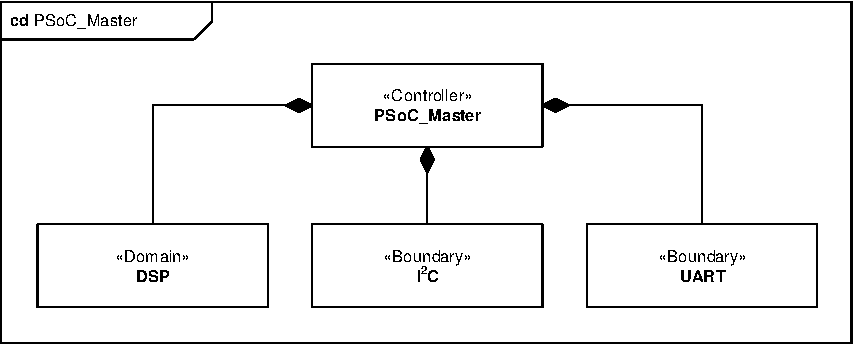
\includegraphics[width={\textwidth}*4/5, trim=0 0 0 0, clip=true] {../fig/cd_PSoC_master_simple.pdf}
\caption{Klassediagram over PSoC Master.}
\label{fig:Master_PSoC_cd}
\end{figure}

Under designet af PSoC Master blev det nøje overvejet hvilke datatyper, der skulle returneres og bruges som parametre i de forskellige metoder.

Ydermere er det generelt i designfasen overvejet, hvordan de forskellige værdier er repræsenteret i binære mønstre og decimalværdier.
Dette er gjort med henblik på at de forskellige klassers metoder skal kunne bruges sammen, så at eksempelvis returværdien fra \texttt{getLight()} i \IIC klassen kan sættes direkte ind i \texttt{inputLight()} i DSP klassen.

\subsubsection{PSoC\_Master Klassen}
\begin{figure}[h]
\centering 
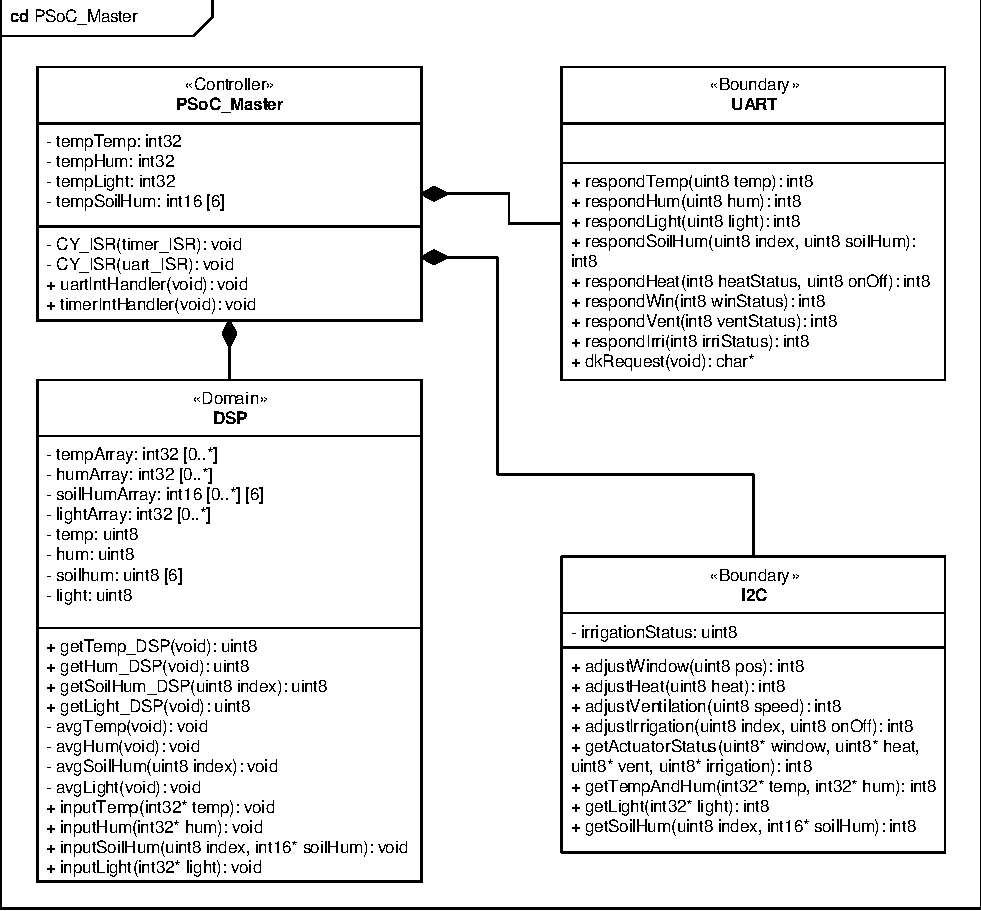
\includegraphics[width=\textwidth * 2/5, trim=15 282 269 31, clip=true] {../fig/cd_PSoC_master.pdf}
\caption{PSoC\_Master klassen.}
\label{fig:Master_PSoC_klasse}
\end{figure}

På Figur \ref{fig:Master_PSoC_klasse} ses et diagram for PSoC\_Master klassen.
Formålet og tanken bag klassen er, at denne skal styre al funktionalitet i PSoC Master blokken.
Som udgangspunkt var det tænkt, at al funktionalitet skulle ligge i de to interrupt service rutiner (\texttt{timer\_ISR} og \texttt{uart\_ISR}). 
Dette viste sig sidenhen at være uhensigtsmæssigt, da der ofte opstod konflikter mellem de to interrupt service rutiner.
Der blev derfor lavet to yderligere metoder, nemlig \texttt{uartIntHandler()} og \texttt{timerIntHandler()} til at håndtere funktionaliteten for hhv. UART og timer.
Dette viste sig at løse en del af problemerne.

Der er senere erfaret, at samhørigheden kunne være større ved at lade interrupt service rutinerne ligge i deres respektive klasser, da de er tæt knyttet til hardwaren.
Dog blev de lagt i PSoC\_Master klassen, da de oprindeligt var tiltænkt at også indeholde al funktionaliteten.
\subsubsection{I2C Klassen}	\label{sec:I2C_design}

Der er designet en \IIC protokol (side \pageref{P-sec:I2C_protokol} i dokumentationen), som dækker over samtlige kommandoer der kan sendes.
Protokollen er designet med rige udvidelsesmuligheder, således er kommandoerne mulige at ændre, hvis der stødes på problemer med nogle af dem, eller hvis der er behov for at udvide funktionaliteten.

\begin{figure}[h]
\centering 
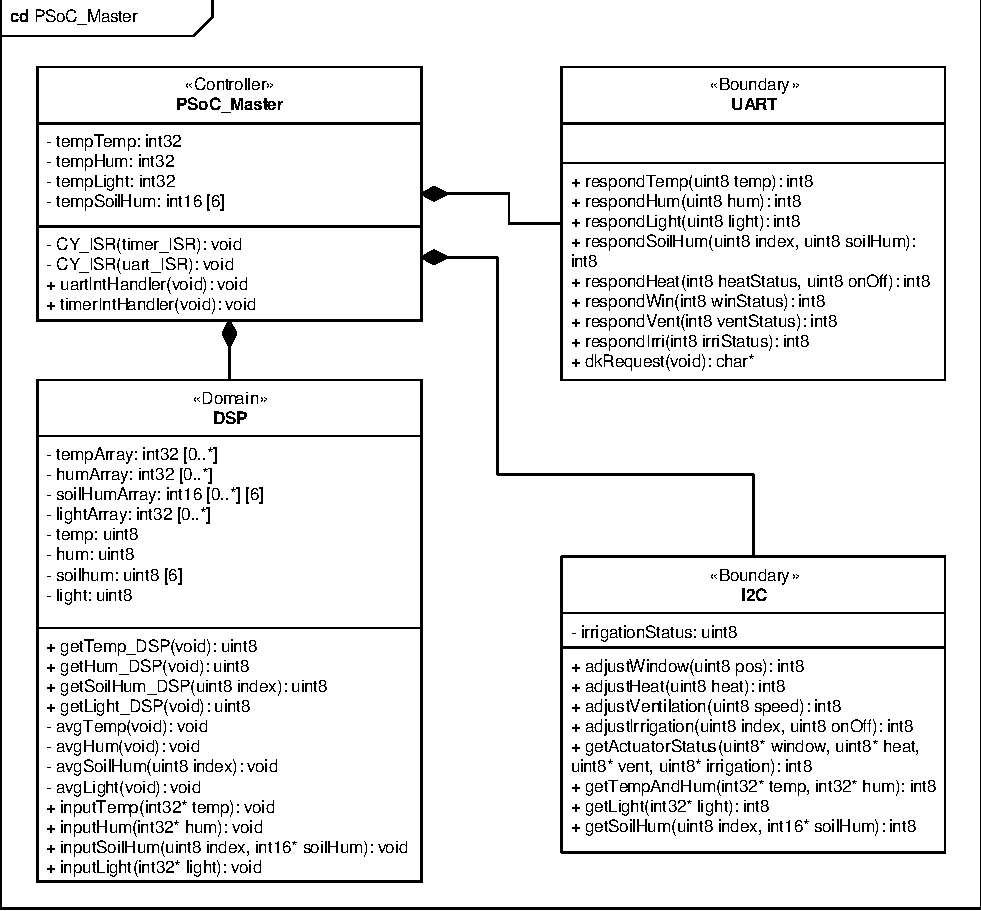
\includegraphics[width=\textwidth * 2/5, trim=269 27 17 267, clip=true] {../fig/cd_PSoC_master.pdf}
\caption{I2C klassen.}
\label{fig:i2C_klasse}
\end{figure}

Klassen \IIC står for indhentning og afsending af data fra/til hhv. sensorer og aktuatorer. Som det kan ses i klassediagrammet på Figur \ref{fig:i2C_klasse} er der designet metoder, hvis navne svarer til kommandoer. Formålet med klassen er, at varetage kommunikation på \IIC bussen. Eksempelvis varetager \texttt{adjustHeat()} metoden den kommunikation til Aktuator-slaven, når der skal slukkes eller tændes for varmelegemet. Metodens returværdi afspejler om kommunikationen gik godt, og at slaven har forstået beskeden.\clearpage
\subsubsection{DSP Klassen}

DSP klassen har til formål at indsamle og behandle den data, som alle sensorerne leverer. Klassen er designet så den er meget skalerbar, da den kan opsættes til at gemme de alt imellem én og flere hundrede seneste målinger for hver sensor. Ligeledes kan den justeres til hvor mange af de gemte målinger der skal være valide, for at måleresultatet er gyldigt og kan sendes til DevKit8000 frem for en fejlmeddelelse. Ud over denne vurdering er klassen designet, så den foretager et gennemsnit af alle de gemte datapunkter for en bestemt sensor, og gemmer den i en variabel (fx \texttt{temp}) der er klar til at blive hentet ud af klassen og sendt direkte til DevKit8000.

\begin{figure}[ht]
\centering 
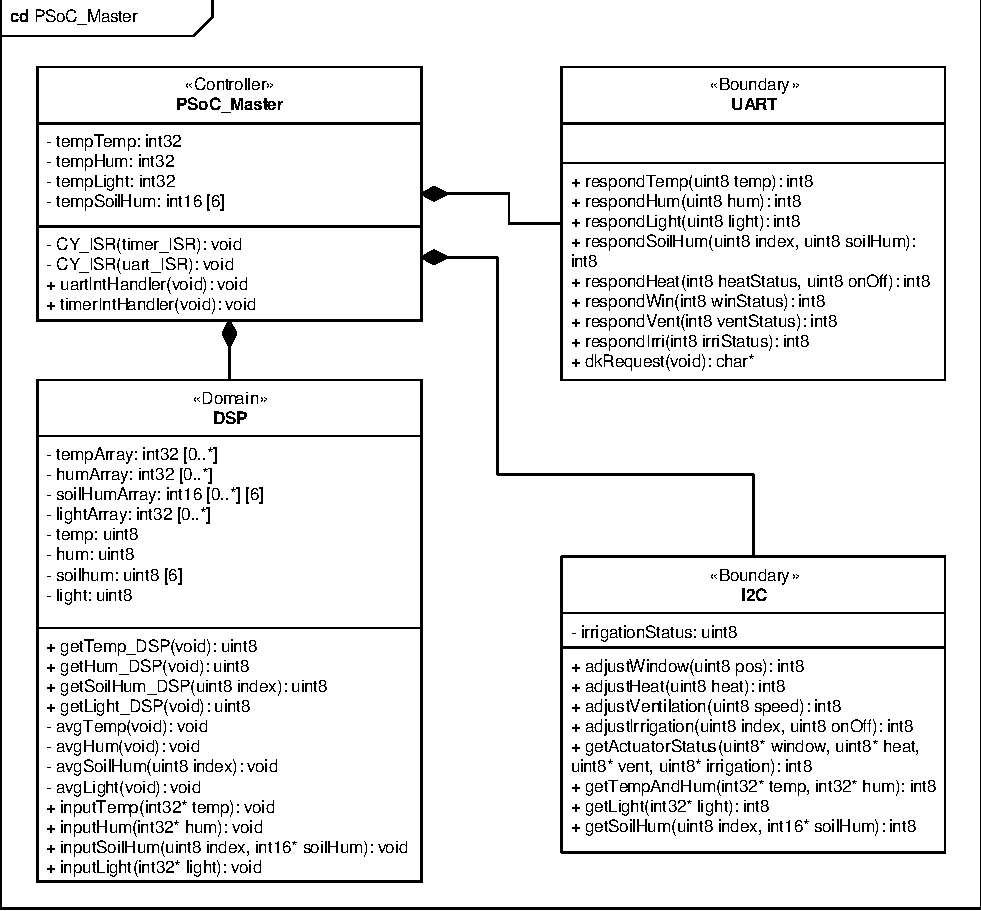
\includegraphics[width=\textwidth * 2/5, trim=15 13 268 182, clip=true] {../fig/cd_PSoC_master.pdf}
\caption{DSP klassen.}
\label{fig:DSP_klasse}
\end{figure}

På Figur \ref{fig:DSP_klasse} ses et klassediagram over DSP klassen. Der er private datamembers både i form af arrays og almindelige variable til at gemme hhv. rå sensordata og klargjorte data. Det kan ses, at \texttt{soilHumArray} er et to-dimensionalt array, da det herved er nemmere at implementere behandlingen af jordfugt-data ved for-løkker.

Vejen for et datapunkt ind og ud af klassen kan beskrives ved et par punkter. Her er et eksempel med temperaturen:

\begin{enumerate}\itemsep1pt \parskip0pt \parsep0pt
\item Den målte temperaturdata hentes direkte fra sensoren og gemmes i DSP klassen ved at kalde \texttt{inputTemp()} metoden fra PSoC Master klassen (styret af en timer).

\item Når \texttt{inputTemp()} kaldes, gemmes datapunktet i \texttt{tempArray} og den private metode \texttt{avgTemp()} kaldes herefter automatisk.

\item Metoden \texttt{avgTemp()} kontrollerer, om der er nok valide datapunkter, tager gennemsnittet over alle punkterne i \texttt{tempArray}, konverterer data'en til formatet der passer til UART protokollen og gemmer resultatet i \texttt{temp}.

\item Når DevKit8000 anmoder om temperaturen, kan \texttt{getTemp\_DSP()} blot kaldes for at få den færdigbehandlede temperatur.

\end{enumerate}

Det detaljerede design med klassebeskrivelser m.m. kan findes i afsnit \ref{P-sec:DSP_class_design} \nameref{P-sec:DSP_class_design} på side \pageref{P-sec:DSP_class_design} i dokumentationen.\clearpage
\subsubsection{UART Klassen}

Grænsefladen mellem DevKit8000 og PSoC Masteren blev valgt som UART, grundet tidligere erfaringer med denne type af kommunikation. Der blev designet en UART-protokol (nærmere beskrevet i afsnit \ref{P-sec:UART_protokol} \nameref{P-sec:UART_protokol} på side \pageref{P-sec:UART_protokol} i dokumentationen), som beskriver kommandoer der er nødvendige for systemet. UART klassen virker således som en driver, der håndterer kommunikationen med DevKit8000.

\begin{figure}[h]
\centering 
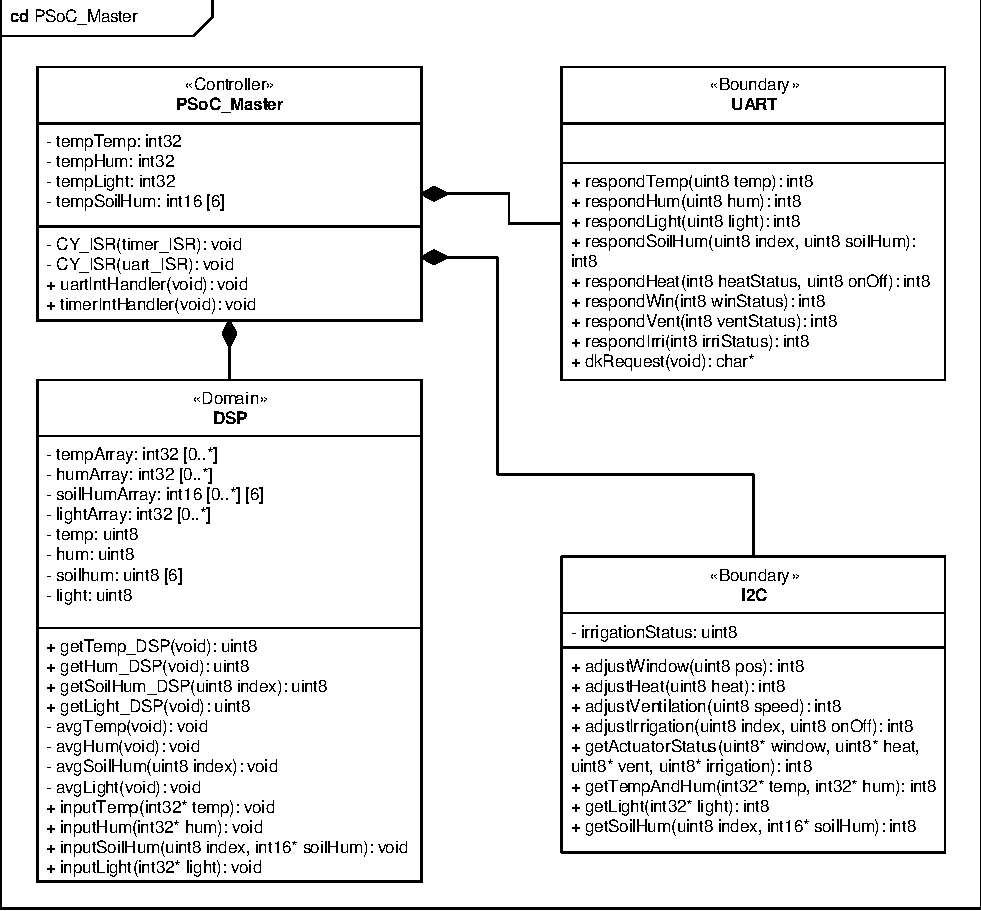
\includegraphics[width=\textwidth * 2/5, trim=269 253 17 30, clip=true] {../fig/cd_PSoC_master.pdf}
\caption{UART klassen}
\label{fig:UART_klasse}
\end{figure}

På Figur \ref{fig:UART_klasse} ses klassediagrammet for UART. Der er designet en public metode, \texttt{dkRequest()}, der sørger for at læse den data, der måtte stå i UART bufferen. Tanken er, at denne metode kaldes fra PSoC Master klassen, når der registres et interrupt. Alle \texttt{respond}-metoderne kaldes med en parameter, der valideres af metoden og hvis denne er gyldig (ikke nul), sendes en passende besked til DevKit8000 jf. UART-protokollen. Eksempelvis sendes \texttt{'X'+'T'}, hvis der er en ugyldig temperatur i DSP-klassens' \texttt{temp} variabel og \texttt{'T'+80} hvis der er målt $20^{\circ}$C med temperatursensoren.
\section{Breakoutboards} \label{sec:breakoutboards}

Da AutoGreen er tiltænkt at skulle monitorere temperatur, luftfugtighed og lysintensitet, blev der valgt nogle sensorer der kunne foretage målinger af disse variable. 

Temperatur- og luftfugtighedssensoren som blev valgt var en \textit{HONEYWELL S\&C  HIH6030-021-001} \cite{lib:TempHum_DS}. Sensoren følger en standard \IIC-protokol og det er nødvendigt at tage hensyn til \IIC-klokkens hastighed samt spændingen på \IIC-bussen, så det er muligt for alle enheder på bussen at kommunikere. Fra producenten har sensoren fået en standard adresse, som skal bruges til kommunikation med enheden.

Lyssensoren der blev valgt var en \textit{Intersil ISL29010IROZ}\cite{lib:LightSens}. Lysfølsomheden kan ændres i sensoren ved at ændre en reference vha. forskellige modstandsstørrelser. Intensiteten af lyset måles i lumen, og sensoren kan måle fra 0 til 128.000 lumen, hvilket passer fint til drivhuset, som kan stå både i mørke og i stærk sollys. Som udgangspunkt oplyser databladet at sensoren fungerer bedst som vist i multisimdiagrammet i Figur \ref{fig:temp_fugt_lys_design}.

Størrelsen på sensorene gør dem meget svære at arbejde med, så der blev designet et breakoutboard til hver sensor. 
Både Temp/Luftfugt og Lyssensoren er af SOIC typen og meget små, så der er anvendt Multisim og Ultiboard til design af breakoutboards, så interfacing med sensorerne blev gjort væsentligt nemmere. Kredsløbene for breakout boards kan ses i Figur \ref{fig:temp_fugt_lys_design}. 

\begin{figure}[h]
\centering
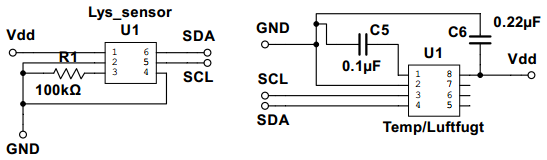
\includegraphics[trim=0 0 0 0, clip=true]{../fig/TempOgLys.png}
\caption{Design af temp/luftfugtsensor og lyssensor breakoutboards.}
\label{fig:temp_fugt_lys_design}
\end{figure}

Alle komponenters værdier fra billederne er taget fra sensorernes datablade.

\clearpage

\clearpage